% vim: set tw=78 aw:
\documentclass{beamer}

\usepackage[utf8x]{inputenc} % diacritice
\usepackage[romanian]{babel}
\usepackage{color}			 % highlight
\usepackage{alltt}			 % highlight
\usepackage{code/highlight}	 % highlight
\usepackage{hyperref}        % folositi \url{http://...}
% sau \href{http://...}{Nume Link}
\mode<presentation>
\usetheme{CDL}

% Titlul nu foloseşte Unicode pentru că e o problemă căreia nu i-am dat de
% cap.
\title[Documentatia]{Documentatia}
\subtitle{CDL - Cursul 4}
\institute[ROSEdu]{ROSEdu}
\author[Adrian|Victor]{Victor Cărbune - Adrian Scoică\\(\small victor@rosedu.org - adrian.sc@rosedu.org)}

\begin{document}

% Slide-urile cu mai multe părţi sunt marcate cu textul (cont.)
\setbeamertemplate{frametitle continuation}[from second]
% Arătăm numărul frame-ului
\setbeamertemplate{footline}[frame number]

\frame{\titlepage}

\begin{frame}
\tableofcontents
\end{frame}

% NB: Secţiunile nu sunt marcate vizual, ci doar apar în cuprins.
\section{Introducere}

\begin{frame}{Documentația software}
	Ce este?
	\pause
	\begin{itemize}
		\item Text 
		\pause
		\item Tutoriale
		\pause
		\item Metainformații 
		\pause
	\end{itemize} 
	... care însoțesc un produs software. \pause \\
	Pe cine vizează?
	\pause
	\begin{itemize}
		\item Proiectanți (Requirements, API)
		\pause
		\item Dezvoltatori (API, SDK)
		\pause
		\item Utilizatori (Manuale, Tutoriale)
	\end{itemize}
	
\end{frame}

\begin{frame}{The ugly truth}
\begin{center}
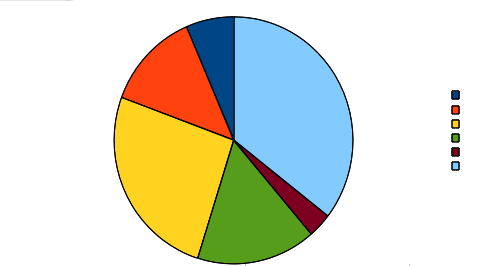
\includegraphics[height=5.5cm, width=11cm]{Step1.png}
\end{center}
\end{frame}

\begin{frame}{The ugly truth}
\begin{center}
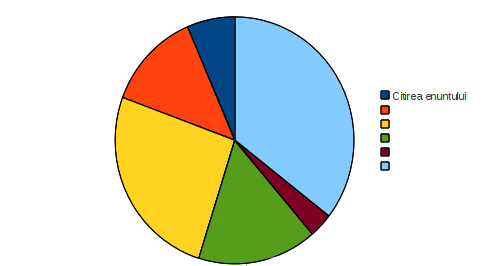
\includegraphics[height=5.5cm, width=11cm]{Step2.png}
\end{center}
\end{frame}

\begin{frame}{The ugly truth}
\begin{center}
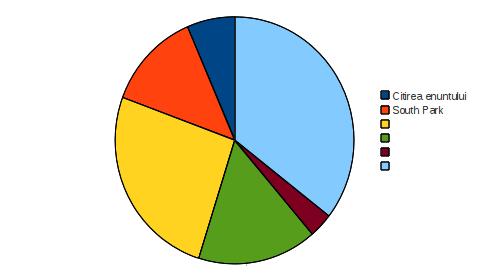
\includegraphics[height=5.5cm, width=11cm]{Step3.png}
\end{center}
\end{frame}

\begin{frame}{The ugly truth}
\begin{center}
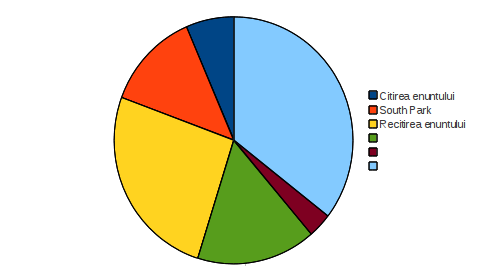
\includegraphics[height=5.5cm, width=11cm]{Step4.png}
\end{center}
\end{frame}

\begin{frame}{The ugly truth}
\begin{center}
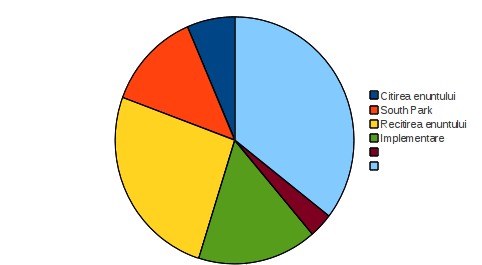
\includegraphics[height=5.5cm, width=11cm]{Step5.png}
\end{center}
\end{frame}

\begin{frame}{The ugly truth}
\begin{center}
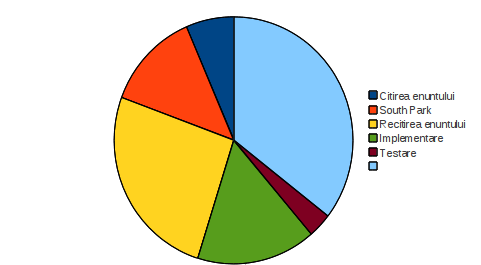
\includegraphics[height=5.5cm, width=11cm]{Step6.png}
\end{center}
\end{frame}

\begin{frame}{The ugly truth}
\begin{center}
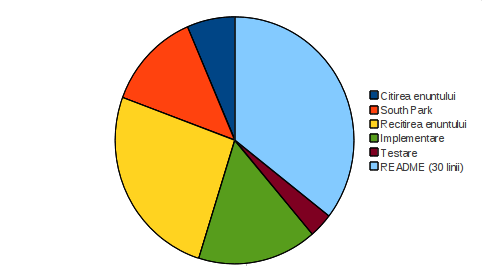
\includegraphics[height=5.5cm, width=11cm]{Step7.png}
\end{center}
\end{frame}

\begin{frame}{The ugly truth}
	Programatorii detestă să scrie documentație.
	\pause
	\begin{itemize}
		\item "Pentru că {\bf pare} timp mort"
		\pause
		\item "Pentru că {\bf PCTTOR\_BK\_TAG\_OP\_CLCL} este un nume de constanta sugestiv"
		\pause
		\item "Pentru că oricum este evident ce face {\bf int prior\_load(const std::priority\_queue$<$SCRTok::Lexem, std::vector$<$SCRTok::Lexem$>$, std::greater$<$SCRTok::Lexem$>$ $>$\& lex);}
		\pause
		\item "Pentru că oricum o să fac modificări mai târziu"
		\pause
	\end{itemize}
\end{frame}

\begin{frame}{Consecințele}
  \begin{itemize}
  \pause
  \item Codul este greu de refolosit, înțeles și modularizat
  \pause
  \item Devine un coșmar să încerci să adaugi funcționalități sau să repari bug-uri
  \pause
  \item Ceilalți programatori evită codul
  \end{itemize}
  \pause
  ... și în cele din urmă, proiectul moare.
\end{frame}

\section{Cum se scrie documentația}

\begin{frame}{Step 1: naming conventions}
	\begin{itemize}
		\item Primul pas către un cod lizibil.
		\pause
		\item Nume scurte și sugestive.
		\pause
			\begin{itemize}
			\item make\_sanwdich\_in\_c();
			\pause
			\item makeSandwichInCamelCase();
			\pause
			\item SandwichClass;
			\pause
			\end{itemize}
		\item {\bf Uniformitatea} este cuvântul cheie.
		\pause
	\end{itemize}
	Alte convenții (doar câteva):
	\begin{itemize}
		\item CONSTANTELE\_IN\_UPPER\_CASE // (SI MACRO-URILE)
		\pause
		\item \_membrii \_privati \_cu \_underscore \_în \_față
		\pause
		\item {\bf pTable} este un {\bf p}Pointer la un Table
		\pause
		\item {\bf hTable} este un {\bf h}Handler pentru un Tabel
		\pause
		\item "{\bf line}" este mai bine decât "{\bf l}"
		\pause
		\item "{\bf index\_to\_line}" este mai rău decât "{\bf l}"
		\pause
	\end{itemize}
\end{frame}

\begin{frame}{Step 2: comentariile}
	\begin{itemize}
		\item {\bf Cel mai important} pas către un cod vizibil.
		\pause
		\item Urmăresc structura logică a codului ({\bf paragrafe})
		\pause
		\item Aduc completări necesare (nu redundante): complexitate, sfaturi, cazuri de eroare
		\pause
		\item Nu trebuie să conțină povești, ASCII art, proverbe,...
		\pause
		\item ... sau înjurături ...
		\pause
	\end{itemize}
	În proiectele mari, este bine să includeți la începutul fișierului un antet cu:
	\begin{itemize}
		\item Versiunea de fișier (cu data curentă)
		\pause
		\item Autorul codului
		\pause
		\item O metodă de contact
		\pause
	\end{itemize}
\end{frame}

\begin{frame}{Step 2: comentariile - câte greșeli vedeți?}
	\noindent
\ttfamily
\hlstd{\hlline{\ \ \ \ 1\ }std}\hlsym{::}\hlstd{ifstream\ }\hlkwd{in}\hlstd{}\hlsym{(}\hlstd{}\hlstr{"joc2.in"}\hlstd{}\hlsym{);\ }\hlstd{}\hlslc{//\ Deschide\ fis\ input}\\
\hlline{\ \ \ \ 2\ }\hlstd{std}\hlsym{::}\hlstd{ofstream\ }\hlkwd{out}\hlstd{}\hlsym{(}\hlstd{}\hlstr{"joc2.out"}\hlstd{}\hlsym{);\ }\hlstd{}\hlcom{/{*}\ Deschide\ fis\ output\ {*}/}\hlstd{}\\
\hlline{\ \ \ \ 3\ }\hlslc{//\ {*}{*}{*}{*}{*}{*}{*}{*}\ ==\ Citirea\ datelor\ ==\ {*}{*}{*}{*}{*}{*}{*}{*}{*}{*}{*}{*}{*}}\\
\hlline{\ \ \ \ 4\ }\hlstd{in\ }\hlsym{$>$$>$\ }\hlstd{N}\hlsym{;\ }\hlstd{}\hlslc{//\ Better\ hope\ the\ s{*}{*}{*}\ doesn't\ fail\ reading}\\
\hlline{\ \ \ \ 5\ }\hlstd{}\hlkwa{for\ }\hlstd{}\hlsym{(}\hlstd{}\hlkwb{int\ }\hlstd{I\ }\hlsym{=\ }\hlstd{}\hlnum{0}\hlstd{}\hlsym{;\ }\hlstd{I\ }\hlsym{$<$\ }\hlstd{N}\hlsym{;\ }\hlstd{I}\hlsym{++)}\\
\hlline{\ \ \ \ 6\ }\hlstd{}\hlstd{\ \ \ \ \ \ \ \ }\hlstd{in\ }\hlsym{$>$$>$\ }\hlstd{tab}\hlsym{{[}}\hlstd{I}\hlsym{{]}.}\hlstd{first\ }\hlsym{$>$$>$\ }\hlstd{tab}\hlsym{{[}}\hlstd{I}\hlsym{{]}.}\hlstd{second}\hlsym{;}\\
\hlline{\ \ \ \ 7\ }\hlstd{}\hlslc{//\ {*}{*}{*}{*}{*}{*}{*}{*}{*}{*}{*}{*}{*}{*}{*}{*}{*}{*}{*}{*}{*}{*}{*}{*}{*}{*}{*}{*}{*}{*}{*}{*}{*}{*}{*}{*}{*}{*}{*}{*}{*}{*}{*}}\\
\hlline{\ \ \ \ 8\ }\hlstd{}\hlslc{//\ This\ would've\ beem\ much\ better\ in\ O(NlogN),\ but}\\
\hlline{\ \ \ \ 9\ }\hlstd{}\hlslc{//\ who\ cares?\ You\ don't\ always\ get\ what\ you\ want\ in\ life...}\\
\hlline{\ \ \ 10\ }\hlstd{}\hlkwa{for\ }\hlstd{}\hlsym{(}\hlstd{}\hlkwb{int\ }\hlstd{w\ }\hlsym{=\ }\hlstd{}\hlnum{1}\hlstd{}\hlsym{;\ }\hlstd{w\ }\hlsym{$<$=\ }\hlstd{}\hlnum{100\ }\hlstd{}\hlcom{/{*}\ maxim\ 100\ linii\ {*}/}\hlstd{}\hlsym{;\ }\hlstd{w}\hlsym{++)\{}\\
\hlline{\ \ \ 11\ }\hlstd{}\hlstd{\ \ \ \ \ \ \ \ }\hlstd{}\hlkwa{for\ }\hlstd{}\hlsym{(}\hlstd{}\hlkwb{int\ }\hlstd{h\ }\hlsym{=\ }\hlstd{}\hlnum{1}\hlstd{}\hlsym{;\ }\hlstd{h\ }\hlsym{$<$=\ }\hlstd{}\hlnum{100}\hlstd{}\hlsym{;\ }\hlstd{h}\hlsym{++)\{}\\
\hlline{\ \ \ 12\ }\hlstd{}\hlstd{\ \ \ \ \ \ \ \ \ \ \ \ \ \ \ \ }\hlstd{}\hlkwa{if\ }\hlstd{}\hlsym{(}\hlstd{w\ }\hlsym{$<$=\ }\hlstd{h}\hlsym{)\ }\hlstd{}\hlslc{//\ If\ w\ $<$=\ h}\\
\hlline{\ \ \ 13\ }\hlstd{}\hlstd{\ \ \ \ \ \ \ \ \ \ \ \ \ \ \ \ \ \ \ \ \ \ \ \ }\hlstd{a}\hlsym{{[}}\hlstd{w}\hlsym{{]}{[}}\hlstd{h}\hlsym{{]}\ =\ }\hlstd{}\hlkwd{count\textunderscore all}\hlstd{}\hlsym{(}\hlstd{w}\hlsym{,}\hlstd{h}\hlsym{);}\\
\hlline{\ \ \ 14\ }\hlstd{}\hlstd{\ \ \ \ \ \ \ \ \ \ \ \ \ \ \ \ }\hlstd{}\hlkwa{else}\\
\hlline{\ \ \ 15\ }\hlstd{}\hlstd{\ \ \ \ \ \ \ \ \ \ \ \ \ \ \ \ \ \ \ \ \ \ \ \ }\hlstd{a}\hlsym{{[}}\hlstd{w}\hlsym{{]}{[}}\hlstd{h}\hlsym{{]}\ =\ }\hlstd{a}\hlsym{{[}}\hlstd{h}\hlsym{{]}{[}}\hlstd{w}\hlsym{{]};}\\
\hlline{\ \ \ 16\ }\hlstd{}\hlstd{\ \ \ \ \ \ \ \ \ \ \ \ \ \ \ \ }\hlstd{}\hlslc{//std::cout\ $<$$<$\ a{[}w{]}{[}h{]}\ $<$$<$\ "\ ";}\\
\hlline{\ \ \ 17\ }\hlstd{}\hlstd{\ \ \ \ \ \ \ \ }\hlstd{}\hlsym{\}}\\
\hlline{\ \ \ 18\ }\hlstd{}\hlsym{\}}\hlstd{}\\
\mbox{}
\normalfont

\end{frame}

\begin{frame}{Step 2: comentariile - un exemplu pozitiv}
	\noindent
\ttfamily
\hlstd{}\hlline{\ \ \ \ 1\ }\hlkwb{int\ }\hlstd{fd\textunderscore src}\hlsym{,\ }\hlstd{fd\textunderscore dst}\hlsym{,\ }\hlstd{rc}\hlsym{,\ }\hlstd{bytesRead}\hlsym{;}\\
\hlline{\ \ \ \ 2\ }\hlstd{}\\
\hlline{\ \ \ \ 3\ }\hlcom{/{*}\ check\ if\ uage\ is\ correct\ {*}/}\hlstd{}\\
\hlline{\ \ \ \ 4\ }\hlkwa{if\ }\hlstd{}\hlsym{(}\hlstd{argc\ }\hlsym{$<$\ }\hlstd{}\hlnum{2\ }\hlstd{}\hlsym{\textbar \textbar \ }\hlstd{argc\ }\hlsym{$>$\ }\hlstd{}\hlnum{3}\hlstd{}\hlsym{)\{}\\
\hlline{\ \ \ \ 5\ }\hlstd{}\hlstd{\ \ \ \ \ \ \ \ }\hlstd{}\hlkwd{printf}\hlstd{}\hlsym{(}\hlstd{}\hlstr{"Wrong\ usage!}\hlesc{$\backslash$n}\hlstr{"}\hlstd{}\hlsym{);}\\
\hlline{\ \ \ \ 6\ }\hlstd{}\hlstd{\ \ \ \ \ \ \ \ }\hlstd{}\hlkwa{return\ }\hlstd{}\hlnum{0}\hlstd{}\hlsym{;}\\
\hlline{\ \ \ \ 7\ }\hlstd{}\hlsym{\}}\\
\hlline{\ \ \ \ 8\ }\hlstd{}\\
\hlline{\ \ \ \ 9\ }\hlcom{/{*}\ open\ source\ file\ for\ reading\ {*}/}\hlstd{}\\
\hlline{\ \ \ 10\ }\\
\hlline{\ \ \ 11\ }\hlkwa{if\ }\hlstd{}\hlsym{(}\hlstd{argc\ }\hlsym{==\ }\hlstd{}\hlnum{3}\hlstd{}\hlsym{)\ \{}\\
\hlline{\ \ \ 12\ }\hlstd{}\hlstd{\ \ \ \ \ \ \ \ }\hlstd{}\hlcom{/{*}\ redirect\ stdout\ to\ destination\ file\ {*}/}\hlstd{}\\
\hlline{\ \ \ 13\ }\hlsym{\}}\\
\hlline{\ \ \ 14\ }\hlstd{}\\
\hlline{\ \ \ 15\ }\hlcom{/{*}\ read\ from\ file\ and\ print\ to\ stdout\ {*}/}\hlstd{}\\
\hlline{\ \ \ 16\ }\\
\hlline{\ \ \ 17\ }\hlcom{/{*}\ close\ file\ {*}/}\hlstd{}\\
\mbox{}
\normalfont

\end{frame}

\section{Doxygen}

\begin{frame}{Step 3: Doxygen}
	\begin{itemize}	
		\item Este dificil să scriem documentația de la 0, separat de cod.
		\pause
		\item Am vrea ca documentația să fie generabilă din surse.
		\pause
		\item Am vrea un limbaj simplu prin care să legăm explicațiile de elemente din cod.
		\pause
		\item Am vrea ca documentația să nu interacționeze cu codul compilabil (=$>$ comentarii).
		\pause
		\item Am vrea o solutie uniformă pentru mai multe limbaje: C, C++, Java, PHP, C\#, Perl
		\pause
		\item Am vrea documentație generabilă în mai multe limbaje: HTML, LaTeX, RTF
	\end{itemize}
	Doxygen este un utilitar open source flexibil și foarte puternic, dar ușor de folosit. \pause \\
	Parsează codul sursă și interpretează comentariile din el.
\end{frame}

\begin{frame}{Step 3: Sintaxa Doxygen}
	Doxygen analizează acele comentarii care preced declarații sau definiții și au următoarea sintaxă: \\
	\noindent
\ttfamily
\hlstd{}\hlline{\ \ \ \ 1\ }\hlcom{/{*}!}\\
\hlline{\ \ \ \ 2\ }\hlcom{...\ Acesta\ este\ un\ comentariu\ specific\ Qt\ (C++,\ dar\ si\ C)}\\
\hlline{\ \ \ \ 3\ }\hlcom{{*}/}\hlstd{\\
\hlline{\ \ \ \ 4\ }\ }\\
\hlline{\ \ \ \ 5\ }\hlslc{//!\ Acesta\ este\ un\ comentariu\ specific\ Qt\ pe\ o\ singura\ linie}\\
\hlline{\ \ \ \ 6\ }\hlstd{}\\
\hlline{\ \ \ \ 7\ }\hlcom{/{*}{*}\ }\\
\hlline{\ \ \ \ 8\ }\hlcom{}\hlstd{\ \ }\hlcom{{*}\ Acesta\ este\ un\ comentariu\ specific\ Java\ }\\
\hlline{\ \ \ \ 9\ }\hlcom{}\hlstd{\ \ }\hlcom{{*}/}\hlstd{\\
\hlline{\ \ \ 10\ }}\hlstd{\ \ }\hlstd{}\\
\hlline{\ \ \ 11\ }\hlslc{///\ Acesta\ este\ un\ comentariu\ specific\ Java\ pe\ o\ singura\ linie}\\
\hlline{\ \ \ 12\ }\hlstd{}\\
\hlline{\ \ \ 13\ }\\
\mbox{}
\normalfont

\end{frame}

\begin{frame}{Step 3: Sintaxa Doxygen - specficații}
	\noindent
\ttfamily
\hlstd{}\hlline{\ \ \ \ 1\ }\hlcom{/{*}{*}}\\
\hlline{\ \ \ \ 2\ }\hlcom{{*}\ Descriere\ detaliata\ a\ functiei}\\
\hlline{\ \ \ \ 3\ }\hlcom{{*}\ @brief\ Descriere\ pe\ scurt\ a\ functiei}\\
\hlline{\ \ \ \ 4\ }\hlcom{{*}\ @param\ x\ Descrierea\ parametrului\ x}\\
\hlline{\ \ \ \ 5\ }\hlcom{{*}\ @param\ y\ Descrierea\ parametrului\ y}\\
\hlline{\ \ \ \ 6\ }\hlcom{{*}\ @return\ Descrierea\ valorii\ returnate}\\
\hlline{\ \ \ \ 7\ }\hlcom{}\\
\hlline{\ \ \ \ 8\ }\hlcom{{*}\ Un\ $<$b$>$exemplu$<$/b$>$\ folosire\ form.\ matematice\ in\ text:}\\
\hlline{\ \ \ \ 9\ }\hlcom{{*}\ Distanta\ e\ /f\$$\backslash$sqrt\{\ (x\textunderscore 2{-}x\textunderscore 1)\textasciicircum 2\ +\ (y\textunderscore 2\ {-}\ y\textunderscore 1)\textasciicircum 2\ \}/f\$}\\
\hlline{\ \ \ 10\ }\hlcom{{*}\ Daca\ dorim\ ca\ formula\ sa\ fie\ centrata\ pe\ o\ singura\ linie:}\\
\hlline{\ \ \ 11\ }\hlcom{{*}\ /f{[}}\\
\hlline{\ \ \ 12\ }\hlcom{{*}\ $\backslash$sqrt\{\ (x\textunderscore 2{-}x\textunderscore 1)\textasciicircum 2\ +\ (y\textunderscore 2\ {-}\ y\textunderscore 1)\textasciicircum 2\ \}}\\
\hlline{\ \ \ 13\ }\hlcom{{*}\ /f{]}}\\
\hlline{\ \ \ 14\ }\hlcom{{*}\ Observatie:\ toate\ formulele\ trebuie\ sa\ fie\ comenzi\ LaTeX.\ }\\
\hlline{\ \ \ 15\ }\hlcom{{*}\ Trebuie\ ca\ LaTeX\ sa\ fie\ instalat\ pe\ calculator.}\\
\hlline{\ \ \ 16\ }\hlcom{{*}/}\hlstd{}\\
\hlline{\ \ \ 17\ }\hlkwb{double\ }\hlstd{}\hlkwd{distantaInPlan}\hlstd{}\hlsym{(}\hlstd{Point2D}\hlsym{\&\ }\hlstd{x}\hlsym{,\ }\hlstd{Point2D}\hlsym{\&\ }\hlstd{y}\hlsym{);}\hlstd{}\\
\mbox{}
\normalfont

\end{frame}

\begin{frame}{Step 4: Generarea documentatiei cu Doxygen}
	Avem mai intai nevoie de un fisier de configurare pentru doxygen.
	\pause
	\begin{itemize}
		\item Un fisier de configurare se poate obtine cu comanda {\bf doxygen -g fisier\_cofig}
	\end{itemize}
	\pause
	Al doilea pas este editarea fisierului conform cu cerintele noastre.
	\pause
	\begin{itemize}
		\item In final, vom folosi fisierul pentru a genera documentația {\bf doxygen fisier\_config}
	\end{itemize}
	\pause
	\begin{itemize}
		\item {\bf TASK} Descărcați de la adresa http://swarm.cs.pub.ro/\~adrian.sc/doxygen\_task fisierele sursă de C++ și generați documentația aferentă lor.
	\end{itemize}
\end{frame}

\section{Resurse}

\begin{frame}{Resurse}
  \begin{itemize}
  \item http://www-glast.slac.stanford.edu/software/CodeHowTo\_20021202/doxygen/using\_doxygen.htm
  \pause
  \item http://www.devtopics.com/13-tips-to-comment-your-code/
  \pause
  \item http://www.codinghorror.com/blog/2004/11/when-good-comments-go-bad.html  
  \pause
  \vspace{10mm}
  \item Întrebări?
  \end{itemize}
\end{frame}

\begin{frame}{}
\end{frame}

\end{document}
